% =====================================================================
\chapter{Modelo cinemático, jacobiano y modelo 3D}\label{cap:cinematica}

\section{Levantamiento de medidas}
El modelo parte de un levantamiento de la máquina: 20 fotos acotadas (\codigo{modelo-3d/levantamiento/fotos/}), bocetos de las piezas, una planilla de medición imprimible y el manual del fabricante. Después, el equipo replicó el brazo pieza por pieza en \textbf{Autodesk Inventor} (\codigo{global/modelo-3d/inventor/}). Las cotas del mecanismo se tomaron de ese modelo: el script \codigo{levantamiento/medidas\_inventor.py} lee el ensamble exportado a STL (un archivo por pieza, en su posición), ubica los pasadores ajustando circunferencias a los agujeros y escribe \codigo{medidas\_inventor.json}. Cada cota quedó clasificada como \emph{Inventor}, \emph{leída} (medida en la pieza o el boceto) o \emph{SUPUESTO}.

\begin{figure}[H]
\centering
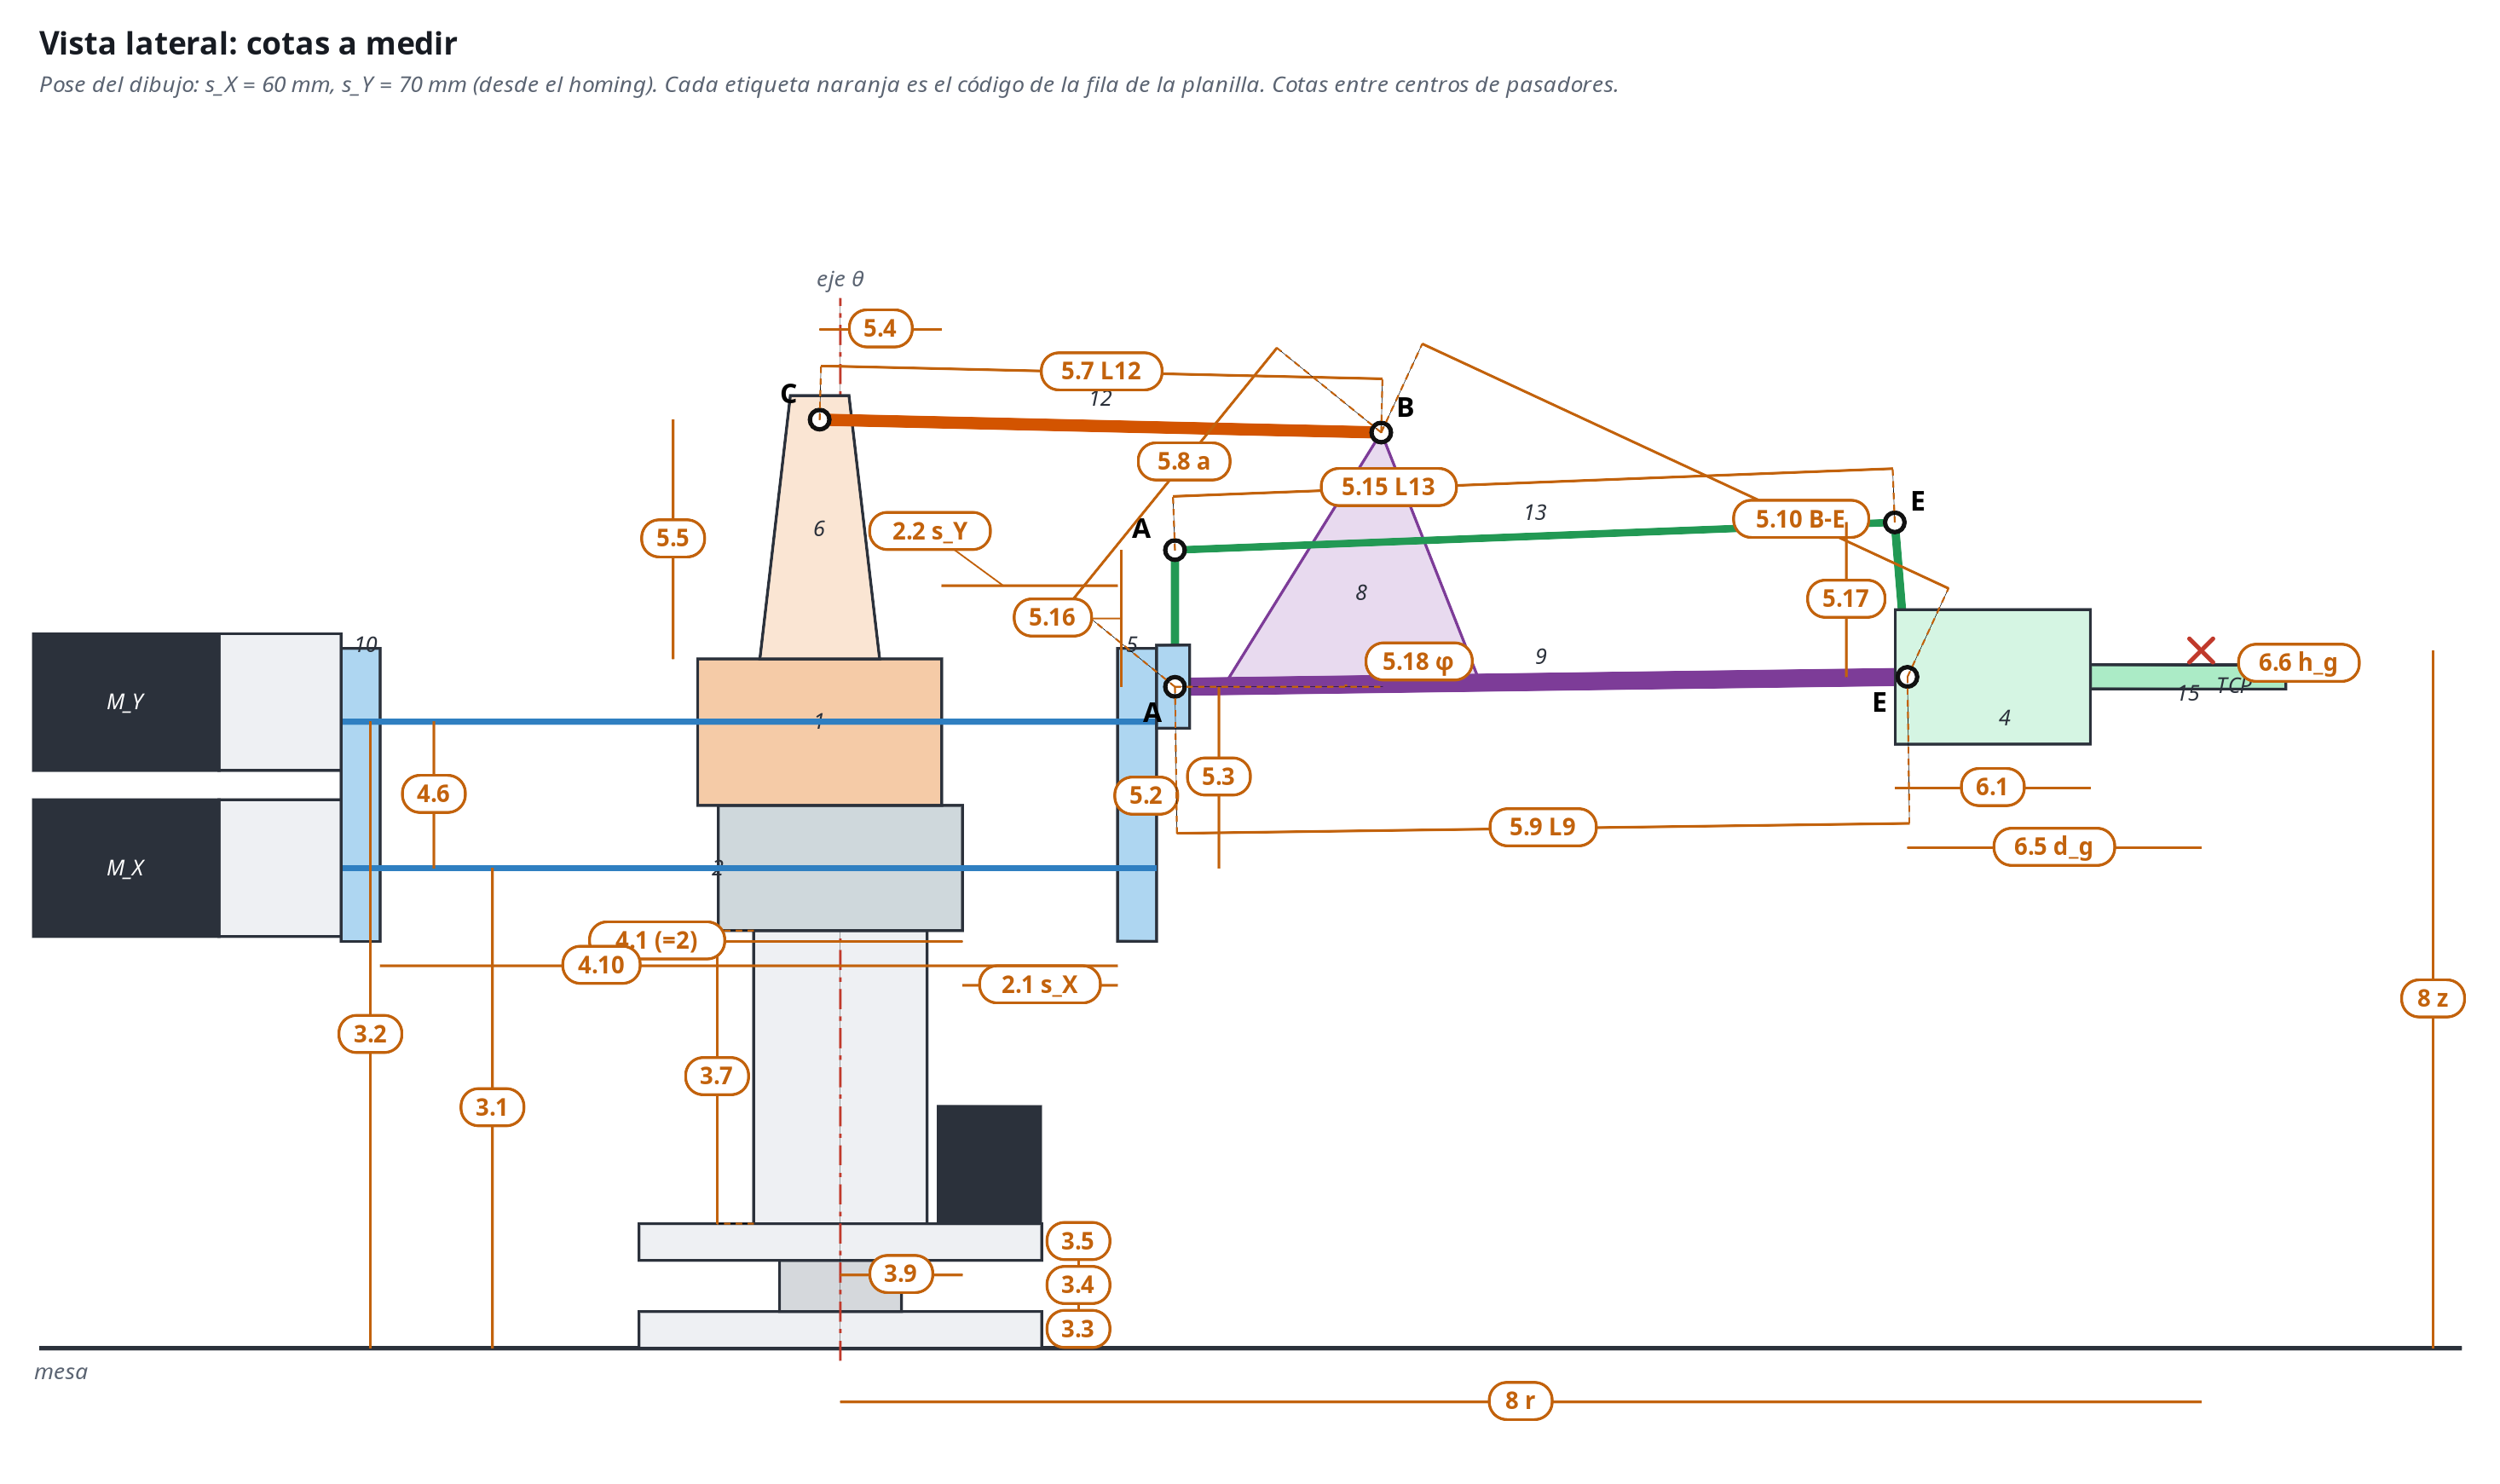
\includegraphics[width=\linewidth]{esquema_medidas_lateral.png}
\caption{Esquema de medidas en vista lateral (\texttt{levantamiento/esquema\_medidas\_lateral.png}).}
\end{figure}

\begin{center}\small
\begin{longtable}{>{\ttfamily}p{2.6cm} r >{\raggedright}p{2cm} >{\raggedright\arraybackslash}p{8cm}}
\toprule
\textbf{\rmfamily Parámetro} & \textbf{Valor} & \textbf{Origen} & \textbf{Significado}\\
\midrule
\endhead
largoGuias & 334 mm & Inventor & entre caras exteriores de las placas (guías Ø16 × 300 entre placas)\\
espesorPlaca & 16 mm & Inventor & placas extremas del bastidor\\
largoBloque, hBloque1, hBloque2 & 100, 51,3, 51,3 mm & Inventor & bloques 1 (carro Y) y 2 (fijo a la columna)\\
sepNiveles & 60 mm & Inventor & distancia entre los centros de los bloques (8,7~mm de luz)\\
holgura & 2 mm & SUPUESTO & distancia bloque--placa en el final de carrera\\
recorridoX, recorridoY & 170 mm & dato del equipo & entre finales de carrera (carrera mecánica libre: 202~mm)\\
a & 134,1 mm & Inventor & balancín A--B\\
beta ($\beta$) & 50,2° & Inventor & ángulo entre A--B y el brazo\\
L12 & 230 mm & Inventor & biela B--C\\
L9 & 300 mm & Inventor & brazo A--E\\
L14, L14E, L13 & 56, 63,5, 295 mm & Inventor & postes A--A$'$ y E--E$'$ y varilla 13: \textbf{no es un paralelogramo}\\
dg, hg & 120,8, 0 mm & Inventor & del pivote E al centro de las mordazas cerradas (TCP)\\
uA, dhA & 23,5, 74,25 mm & Inventor & pivote A: delante de la placa y sobre el centro del bloque 2\\
hC, dhC, uCBloque & 107,9, $-9{,}9$, $-50$ mm & Inventor & pivote C en la escuadra 6, sobre el bloque 1\\
thetaMin, thetaMax & $\pm175$° & SUPUESTO & límite de giro por los cables\\
pasoHusillo & 5 mm & SUPUESTO & husillo SFU1605\\
micropasosXY & 5 (1000 p/vuelta) & leída & DIP de los drivers\\
\bottomrule
\end{longtable}
\end{center}
Todos los parámetros viven en un solo archivo, \codigo{web/js/cinematica.js}; el script \codigo{pruebas\_cinematica.js} los exporta a \codigo{modelo-3d/cinematica/parametros.json} para MATLAB y Python. De ellos se derivan, entre otros: altura del pivote A $h_A = 270{,}9$~mm, posición de la placa delantera con $s_X = 0$, $u_0 = 53{,}55$~mm, y la posición del pivote C respecto de A, $(c_{u0}, c_h) = (-273{,}5;\ 109{,}4)$~mm. Con estas cotas, el modelo reproduce la pose en que se exportó el ensamble de Inventor con un error de 0,4~mm como máximo en todos los pivotes y en la garra (\codigo{levantamiento/comparacion\_inventor.png}).

\section{El mecanismo}
\begin{figure}[H]
\centering
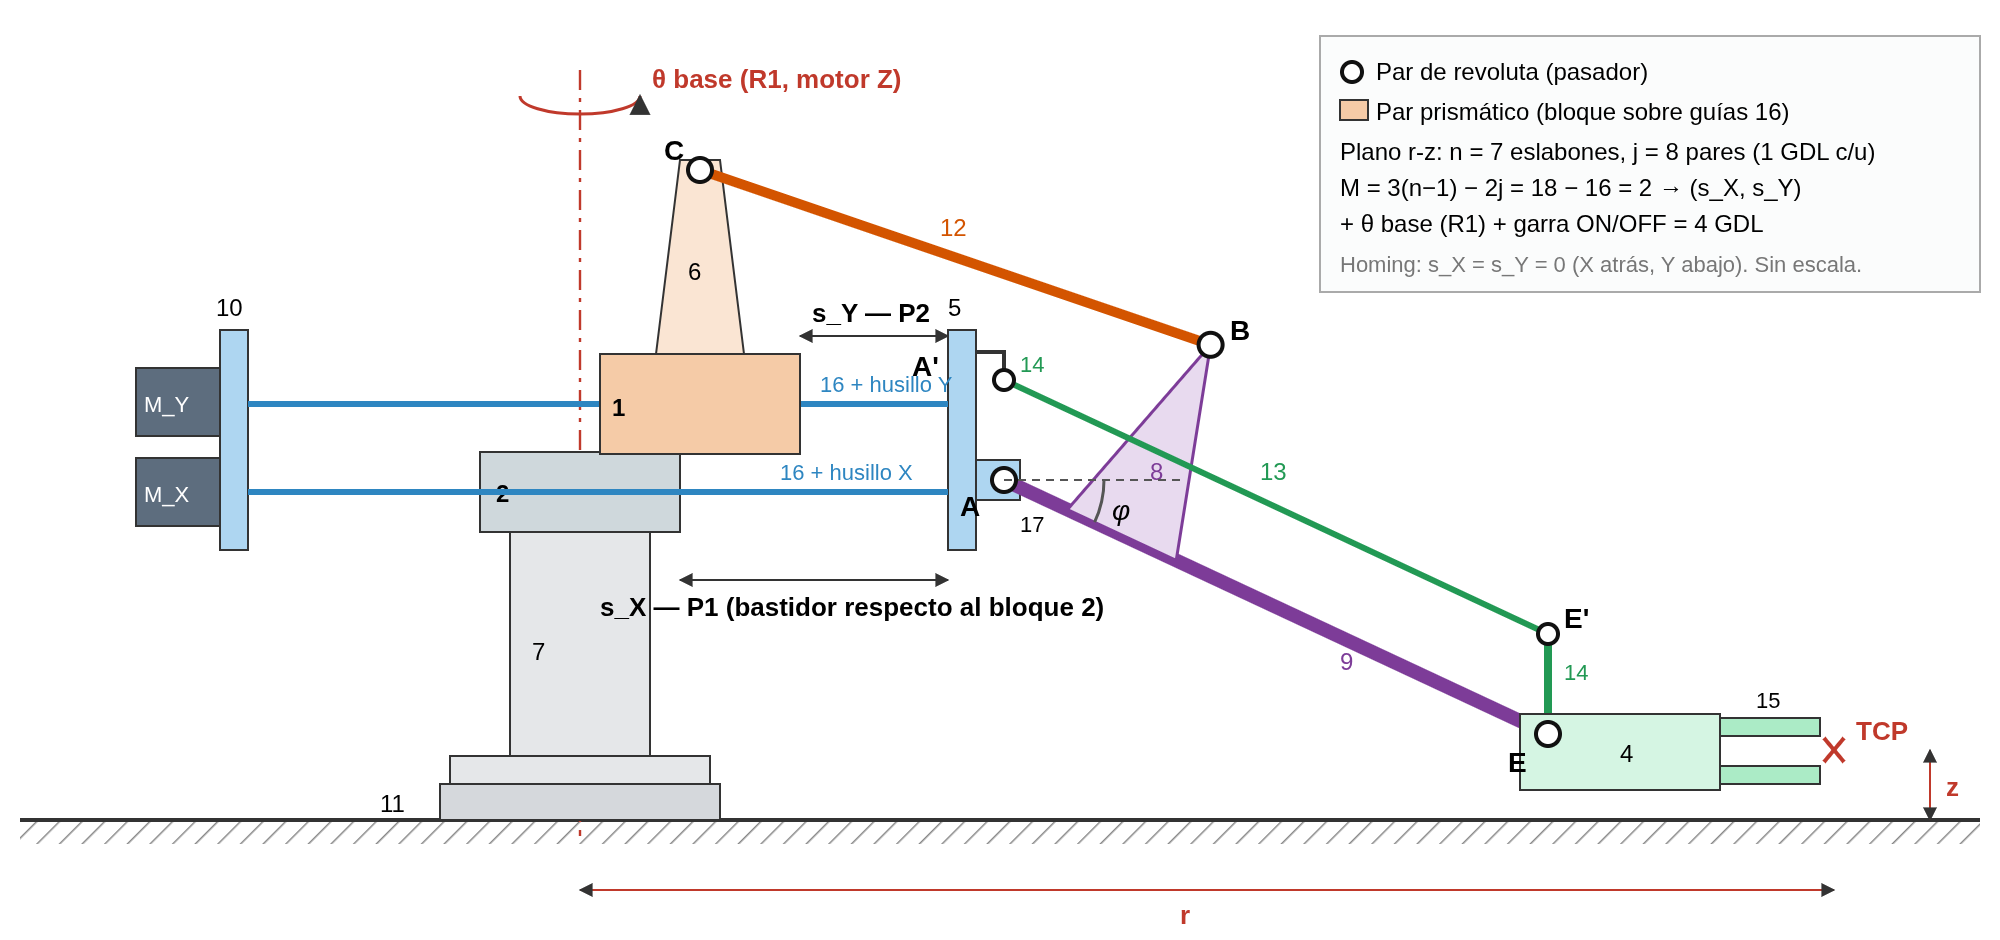
\includegraphics[width=\linewidth]{esquema_cinematico.png}
\caption{Esquema cinemático del brazo (\texttt{modelo-3d/informe/figuras/}).}
\end{figure}

El brazo trabaja en un plano vertical $(r, z)$ que gira con la base:
\begin{itemize}
\item el \textbf{carro X} desplaza todo el bastidor, y con él el pivote A del brazo: cambia el alcance;
\item el \textbf{carro Y} mueve el bloque 1 sobre el bastidor; la biela $L_{12}$ une el pivote C del bloque con el pivote B del balancín A--B, solidario al brazo: al moverse el bloque, el brazo gira un ángulo $\varphi$;
\item la varilla 13 une el poste A$'$ (fijo al bastidor, 56~mm sobre A) con el poste E$'$ de la pinza (63,5~mm sobre E). Como los postes son distintos a propósito, el cuadrilátero A--A$'$--E$'$--E \textbf{no es un paralelogramo}: la pinza se inclina un ángulo $\gamma$ de 0,2° a 13,3° según la altura del brazo.
\end{itemize}

\begin{figure}[H]
\centering
\begin{tikzpicture}[x=1.05cm,y=1.05cm]
\coordinate (A) at (0,0); \coordinate (B) at (1.6,-1.0); \coordinate (C) at (4.3,-0.2);
\coordinate (E) at (6.2,2.3); \coordinate (T) at (7.6,2.0);
\draw[fill=gris] (-2.4,-2.6) rectangle (3.6,-1.9); \node[font=\scriptsize] at (0.6,-2.25) {carro X: desplaza todo el bastidor};
\draw[fill=naranja!20] (3.0,-1.0) rectangle (5.3,0.3); \node[font=\scriptsize] at (4.15,-1.4) {bloque del carro Y};
\draw[ultra thick, grisos] (A) -- (B) node[midway, left, font=\scriptsize]{$a$};
\draw[ultra thick, naranja] (B) -- (C) node[midway, below, font=\scriptsize]{$L_{12}$};
\draw[ultra thick, black] (A) -- (E) node[midway, above left, font=\scriptsize]{brazo $L_9$};
\draw[ultra thick, black] (E) -- (T);
\fill[naranja] (T) circle (0.12); \node[font=\scriptsize, right] at (T) {garra (TCP)};
\foreach \p in {A,B,C,E} {\fill[white] (\p) circle (0.11); \draw (\p) circle (0.11); \node[font=\scriptsize, above] at ($(\p)+(0,0.12)$) {\p};}
\draw[->] (A) ++(1.2,0) arc (0:35:1.2); \node[font=\scriptsize] at (1.6,0.45) {$\varphi$};
\draw[->] (A) ++(0.7,0) arc (0:-32:0.7); \node[font=\scriptsize] at (0.95,-0.25) {$\psi$};
\draw[<->] (3.0,0.7) -- (5.3,0.7) node[midway, above, font=\scriptsize]{$s_Y$};
\draw[<->] (-2.4,-2.9) -- (3.6,-2.9) node[midway, below, font=\scriptsize]{$s_X$};
\end{tikzpicture}
\caption{Esquema simplificado: lazo A--B--C y brazo A--E.}
\end{figure}

\section{Cinemática directa: de los carros a la garra}
Entrada $q = (\theta, s_X, s_Y)$; salida $(X, Y, Z)$ de la garra.

\paragraph{Paso 1: lazo de bielas.} La posición geométrica del bloque es $g = (202 - 2\cdot 2) - s_Y = 198 - s_Y$ (el homing de Y deja el bloque adelante, a 2~mm de la placa). El pivote C queda, respecto de A, en $C = (g + c_{u0},\, c_h) = (g - 273{,}5;\; 109{,}4)$. El pivote B está a distancia $a$ de A y a distancia $L_{12}$ de C: es la intersección de dos circunferencias. Con $d = |C|$,
\[
\psi = \operatorname{atan2}(c_h,\, g + c_{u0}) - \arccos\!\left(\frac{a^2 + d^2 - L_{12}^2}{2\,a\,d}\right),
\]
eligiendo el signo del montaje real (B por debajo de la recta A--C). El ángulo del brazo es $\varphi = \psi - \beta$.

\paragraph{Paso 2: inclinación de la pinza.} A$'$ está fijo a $L_{14}$ sobre A. E$'$ está en la pinza, en $\mathbf{v} = (u_{E2}, L_{14E}) = (0{,}5;\ 63{,}5)$ desde E cuando la pinza está horizontal. La varilla exige $|E + R(\gamma)\,\mathbf{v} - A'| = L_{13}$. Con $\mathbf{w} = A' - E$:
\[
\gamma = \operatorname{atan2}(w_h, w_u) - \operatorname{atan2}(v_h, v_u) - \arccos\!\left(\frac{|\mathbf{v}|^2 + |\mathbf{w}|^2 - L_{13}^2}{2\,|\mathbf{v}|\,|\mathbf{w}|}\right).
\]

\paragraph{Paso 3: posición de la garra en el plano.} El TCP está a $(d_g, -h_g)$ de E en el marco de la pinza, que está girado $\gamma$:
\[
r = u_0 + u_A + s_X + L_9\cos\varphi + d_g\cos\gamma = 77{,}05 + s_X + 300\cos\varphi + 120{,}8\cos\gamma \quad [\text{mm}]
\]
\[
z = h_A + L_9\sin\varphi + d_g\sin\gamma = 270{,}9 + 300\sin\varphi + 120{,}8\sin\gamma \quad [\text{mm}]
\]

\paragraph{Paso 4: giro de la base.} $X = r\cos\theta$, \ $Y = r\sin\theta$, \ $Z = z$.

\paragraph{Ejemplo resuelto: el homing $q = (0, 0, 0)$.} $g = 198$; $C = (-75{,}5;\ 109{,}4)$, $d = 132{,}9$~mm; $\arccos\frac{134{,}1^2 + 132{,}9^2 - 230^2}{2\cdot134{,}1\cdot132{,}9} = \arccos(-0{,}484) = 118{,}9°$; $\operatorname{atan2}(109{,}4;\ -75{,}5) = 124{,}6°$; $\psi = 5{,}7°$, $\varphi = -44{,}5°$. La pinza queda casi horizontal, $\gamma = 0{,}19°$. Luego $r = 77{,}05 + 0 + 300\cos(-44{,}5°) + 120{,}8\cos 0{,}19° = 411{,}7$~mm y $z = 270{,}9 + 300\sin(-44{,}5°) + 120{,}8\sin 0{,}19° = 60{,}9$~mm: la garra queda baja y cerca de la columna.

\begin{figure}[H]
\centering
\begin{minipage}[t]{0.49\linewidth}\centering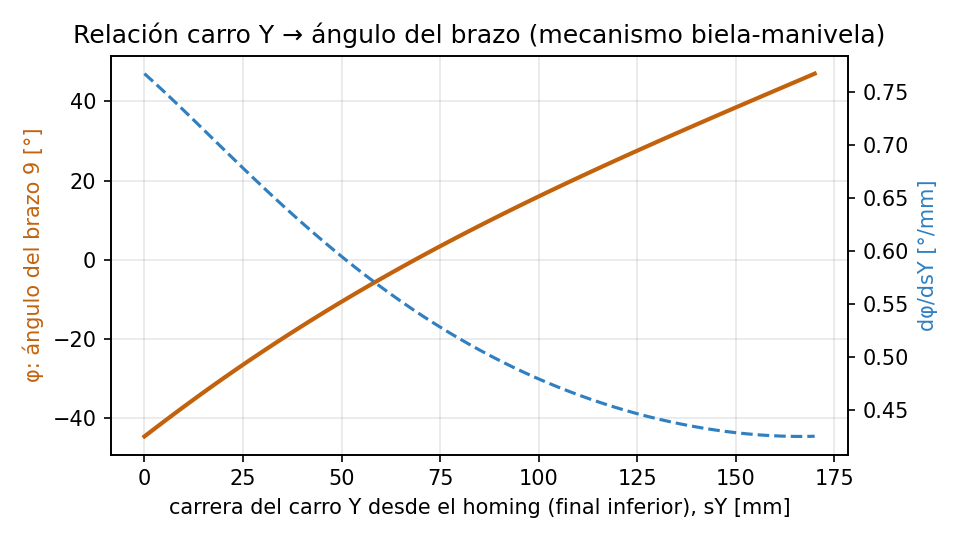
\includegraphics[width=\linewidth]{phi_vs_carro_y.png}\\{\small (a) ángulo del brazo $\varphi$ y su derivada frente a $s_Y$}\end{minipage}\hfill
\begin{minipage}[t]{0.49\linewidth}\centering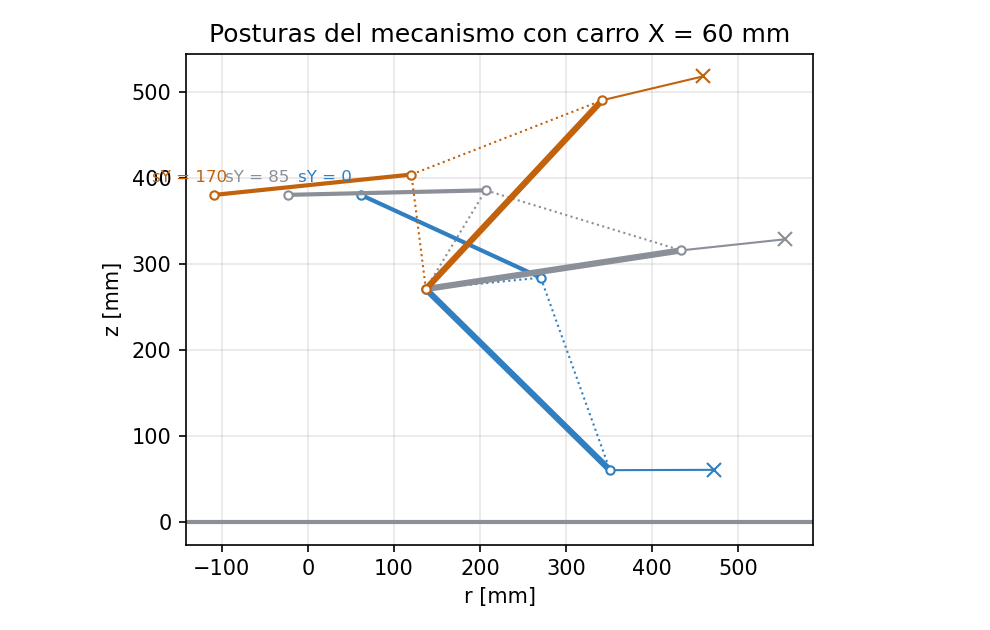
\includegraphics[width=\linewidth]{posturas_mecanismo.png}\\{\small (b) posturas del mecanismo con $s_X = 60$~mm}\end{minipage}
\caption{Relación entre el carro Y y el ángulo del brazo: de $-44{,}5°$ ($s_Y = 0$) a $+47{,}0°$ ($s_Y = 170$~mm), no lineal.}
\end{figure}

\section{Cinemática inversa: de la garra a los carros}
Entrada $(X, Y, Z)$; salida $q$.
\begin{enumerate}
\item $\theta = \operatorname{atan2}(Y, X)$, \ $r = \sqrt{X^2 + Y^2}$. Si hay varias soluciones ($\theta$ y $\theta \pm 360°$), se elige la más cercana a la actual.
\item De la altura: $z(\varphi) = h_A + L_9\sin\varphi + d_g\sin\gamma(\varphi) = Z$. Como la pinza se inclina, ya no hay fórmula cerrada: se resuelve por bisección en cada rama del brazo (adelante y atrás). Si no hay raíz, la altura es inalcanzable.
\item Del alcance: $s_X = r - d_g\cos\gamma - L_9\cos\varphi - u_0 - u_A$.
\item Del lazo: con $\psi = \varphi + \beta$, $B = a(\cos\psi, \sin\psi)$; la biela exige $|B - C| = L_{12}$ con $C = (g - 273{,}5;\ 109{,}4)$:
\[
g = B_x + 273{,}5 \pm \sqrt{L_{12}^2 - (109{,}4 - B_z)^2}, \qquad s_Y = 198 - g,
\]
eligiendo la solución del montaje real.
\item Se descartan soluciones fuera de $0 \le s_X, s_Y \le 170$ o con la pinza chocando con la mesa.
\end{enumerate}

\paragraph{Ejemplo resuelto: garra en $(500, 200, 250)$~mm.} $\theta = \operatorname{atan2}(200, 500) = 21{,}80°$; $r = 538{,}52$~mm; la bisección da $\varphi = -5{,}77°$ con $\gamma = 4{,}39°$; $s_X = 538{,}52 - 120{,}8\cos 4{,}39° - 300\cos(-5{,}77°) - 77{,}05 = 42{,}54$~mm; $\psi = 44{,}43°$, $g = 139{,}78$~mm y $s_Y = 58{,}22$~mm. Comprobación con la directa: vuelve exactamente a $(500{,}000;\ 200{,}000;\ 250{,}000)$.

\section{Jacobiano y linealización}\label{sec:jacobiano}
El jacobiano relaciona pequeños movimientos de los ejes con pequeños movimientos de la garra:
\[
\Delta\mathbf{p} \approx J(q)\,\Delta q, \qquad
J = \frac{\partial(X, Y, Z)}{\partial(\theta, s_X, s_Y)} =
\begin{bmatrix}
-r\sin\theta & \cos\theta & \cos\theta\,\dfrac{\partial r}{\partial s_Y}\\[6pt]
r\cos\theta & \sin\theta & \sin\theta\,\dfrac{\partial r}{\partial s_Y}\\[6pt]
0 & 0 & \dfrac{\partial z}{\partial s_Y}
\end{bmatrix},
\]
con $\dfrac{\partial r}{\partial s_Y} = \left(-L_9\sin\varphi - d_g\sin\gamma\,\dfrac{d\gamma}{d\varphi}\right)\dfrac{d\varphi}{ds_Y}$ y $\dfrac{\partial z}{\partial s_Y} = \left(L_9\cos\varphi + d_g\cos\gamma\,\dfrac{d\gamma}{d\varphi}\right)\dfrac{d\varphi}{ds_Y}$. Como intervienen dos lazos (biela y varilla), \codigo{cinematica.js} calcula $J$ por diferencias centradas; la prueba lo compara con otras diferencias finitas independientes (error $< 10^{-6}$). Esta es la \textbf{linealización} del brazo alrededor de un punto de operación que pide la guía de laboratorio para la Fase 2: cerca de $q_0$, el brazo se comporta como el sistema lineal $\Delta\mathbf{p} = J(q_0)\Delta q$.

\begin{center}\small
\begin{longtable}{>{\raggedright}p{3cm} >{\centering}p{6.3cm} r r r}
\toprule
\textbf{Punto $q$} & \textbf{$J$ ($\theta$ en rad, mm/mm)} & \textbf{$|\det J|$} & \textbf{$d\varphi/ds_Y$} & \textbf{$\mu$}\\
\midrule
\endhead
$(0°, 0, 0)$ homing & $\begin{bmatrix}0 & 1 & 2{,}817\\ 411{,}7 & 0 & 0\\ 0 & 0 & 3{,}062\end{bmatrix}$ & 1261 & 0,767~°/mm & 30,4°\\[14pt]
$(0°, 85, 85)$ centro & $\begin{bmatrix}0 & 1 & -0{,}412\\ 578{,}8 & 0 & 0\\ 0 & 0 & 2{,}760\end{bmatrix}$ & 1597 & 0,507~°/mm & 57,5°\\[14pt]
$(30°, 120, 40)$ & $\begin{bmatrix}-302{,}5 & 0{,}866 & 0{,}808\\ 524{,}0 & 0{,}500 & 0{,}466\\ 0 & 0 & 3{,}281\end{bmatrix}$ & 1985 & 0,626~°/mm & 42,4°\\[14pt]
$(0°, 170, 170)$ esquina & $\begin{bmatrix}0 & 1 & -1{,}686\\ 569{,}3 & 0 & 0\\ 0 & 0 & 1{,}770\end{bmatrix}$ & 1008 & 0,425~°/mm & 91,3°\\
\bottomrule
\end{longtable}
\end{center}

\paragraph{Cómo se lee.} En el centro $(0°, 85, 85)$: un milímetro del carro Y sube la garra 2,76~mm y la acerca 0,41~mm; un milímetro del carro X la aleja exactamente 1~mm; un grado de base la desplaza $578{,}8 \cdot \pi/180 = 10{,}1$~mm de lado. Es decir, el carro Y \emph{amplifica} su movimiento en altura casi 3 veces.

\paragraph{Qué tan buena es la linealización.} Comparación con la cinemática exacta desde el centro:
\begin{center}\small
\begin{tabular}{@{}lccc@{}}
\toprule
$\Delta q = (\Delta\theta, \Delta s_X, \Delta s_Y)$ & exacto $\Delta(X, Y, Z)$ [mm] & lineal $J\Delta q$ [mm] & error\\
\midrule
$(0°, 2, 2)$ & (1,13; 0; 5,49) & (1,18; 0; 5,52) & 0,05~mm\\
$(2°, 0, 0)$ & ($-0{,}35$; 20,20; 0) & (0; 20,20; 0) & 0,35~mm\\
$(0°, 10, 10)$ & (4,84; 0; 26,91) & (5,88; 0; 27,60) & 1,25~mm\\
$(5°, 0, -10)$ & (0,77; 50,70; $-28{,}27$) & (4,12; 50,51; $-27{,}60$) & 3,4~mm\\
\bottomrule
\end{tabular}
\end{center}
La aproximación es excelente para movimientos de pocos milímetros y empeora con desplazamientos grandes, sobre todo de la base (el arco no es una recta). Por eso la página recalcula la inversa en cada punto de una trayectoria en lugar de usar solo el jacobiano.

\paragraph{Singularidades y transmisión.} Como $|\det J| = r\,\partial z/\partial s_Y$ y en todo el recorrido $r > 395$~mm y $\partial z/\partial s_Y > 1{,}7$, el determinante nunca se anula: \textbf{no hay singularidades dentro del recorrido}. El \emph{ángulo de transmisión} $\mu$ entre la biela y el balancín (ideal 90°) mide qué tan bien la biela empuja al brazo: vale 30,4° en el homing (transmisión pobre, el carro Y necesita más fuerza) y 91,3° con el brazo arriba.

\section{Espacio de trabajo}
\begin{figure}[H]
\centering
\begin{minipage}[t]{0.56\linewidth}\centering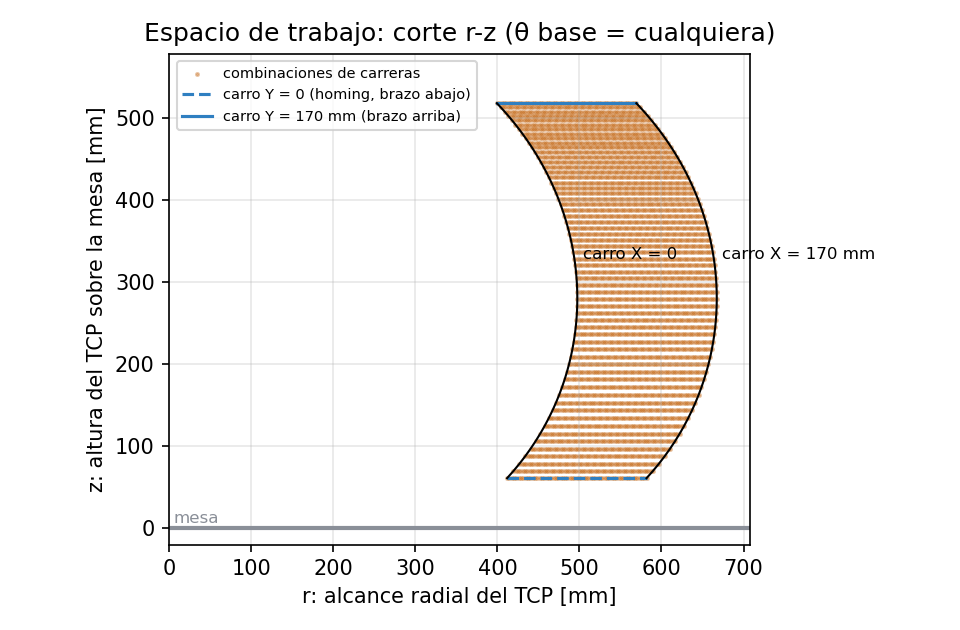
\includegraphics[width=\linewidth]{espacio_trabajo_rz.png}\\{\small (a) corte vertical $(r, z)$}\end{minipage}\hfill
\begin{minipage}[t]{0.42\linewidth}\centering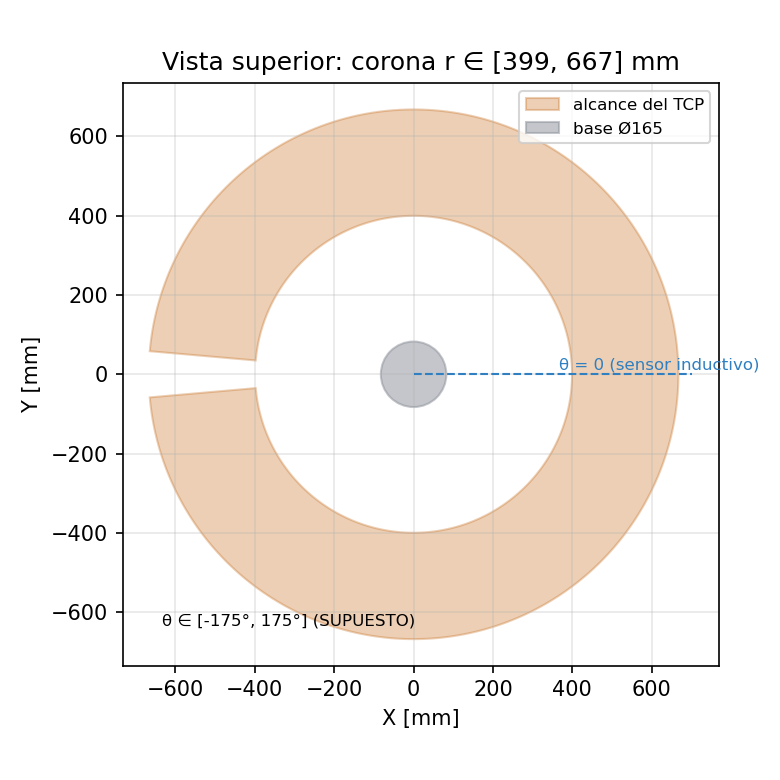
\includegraphics[width=\linewidth]{espacio_trabajo_superior.png}\\{\small (b) vista superior}\end{minipage}
\caption{Espacio de trabajo: una franja curva en el plano vertical que gira con la base; alcance radial de 399 a 667~mm y altura de 61 a 518~mm.}
\end{figure}
Desde el homing (esquina inferior izquierda de la franja), un movimiento vertical de la garra sale de la zona alcanzable: por eso muchos puntos escritos a mano resultan inalcanzables, y la app propone el punto alcanzable más cercano.

\section{Modelo 3D}
El modelo 3D \codigo{global/modelo-3d/brazo\_xk-js1-1.glb} usa las piezas del modelo de Inventor del equipo: el script \codigo{generar\_modelo.js} lee los STL de \codigo{global/modelo-3d/inventor/stl/}, los lleva al marco de cada pieza móvil (base, carros, biela, brazo, pinza, mordazas y varilla) y escribe el GLB. Solo el disco fijo de abajo, que no está en el ensamble de Inventor, se dibuja con primitivas. El visor (three.js) coloca cada pieza según la cinemática directa en cada cuadro, incluida la inclinación $\gamma$ de la pinza. Las figuras se generan con \codigo{global/modelo-3d/dibujar\_modelo.py}.

\begin{figure}[H]
\centering
\begin{minipage}[t]{0.49\linewidth}\centering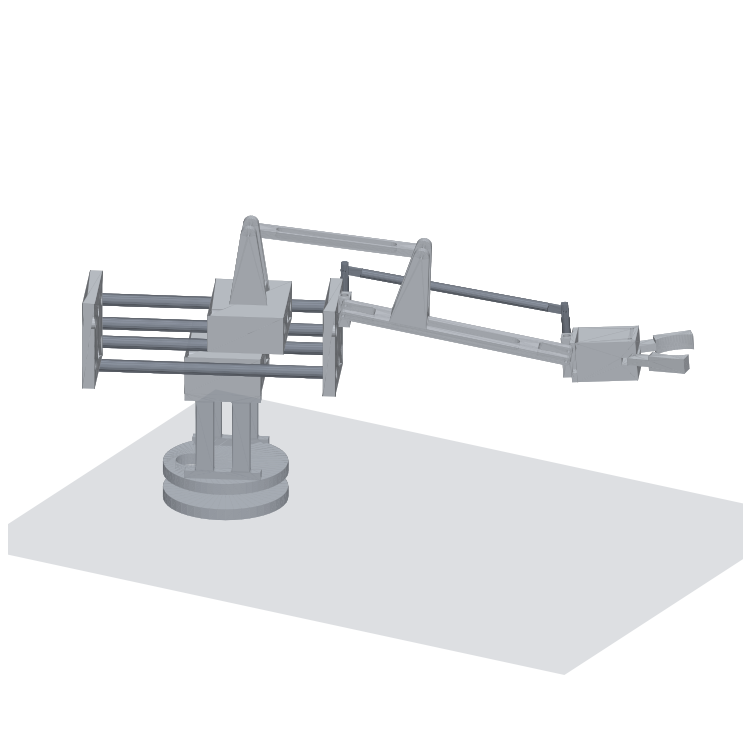
\includegraphics[width=\linewidth]{modelo_3d_isometrica.png}\\{\small (a) isométrica}\end{minipage}\hfill
\begin{minipage}[t]{0.49\linewidth}\centering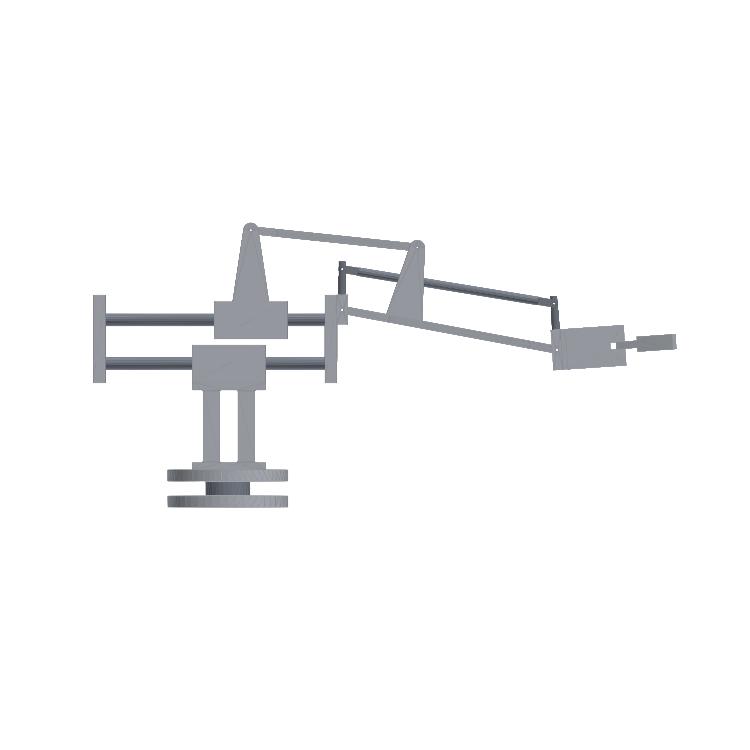
\includegraphics[width=\linewidth]{modelo_3d_lateral.png}\\{\small (b) lateral}\end{minipage}
\caption{Modelo 3D del brazo.}
\end{figure}

\section{Scripts del modelado}
\begin{center}\small
\begin{tabularx}{\linewidth}{>{\raggedright}p{6.2cm} >{\raggedright\arraybackslash}X}
\toprule
\textbf{Archivo} & \textbf{Qué hace}\\
\midrule
\codigo{web/js/cinematica.js} & modelo: parámetros, directa, inversa, jacobiano, espacio de trabajo, pulsos, trayectorias\\
\codigo{modelo-3d/cinematica/pruebas\_cinematica.js} & pruebas: la inversa de la directa devuelve el mismo $q$; exporta \codigo{parametros.json} y \codigo{tabla\_cinematica.csv}\\
\codigo{modelo-3d/cinematica/cinematica\_brazo.m} & la misma cinemática en MATLAB\\
\codigo{modelo-3d/cinematica/graficas\_cinematica.py} & gráficas del informe (espacio de trabajo, $\varphi(s_Y)$, posturas)\\
\codigo{modelo-3d/levantamiento/generar\_esquema\_medidas.py} & esquemas acotados del levantamiento\\
\codigo{modelo-3d/levantamiento/medidas\_inventor.py} & extrae las cotas y los pivotes del STL de Inventor\\
\codigo{global/modelo-3d/generar\_modelo.js} & genera el modelo 3D \codigo{.glb} con las piezas de Inventor\\
\codigo{global/modelo-3d/dibujar\_modelo.py} & dibuja el modelo en una pose (figuras de los informes)\\
\bottomrule
\end{tabularx}
\end{center}

\begin{lstlisting}[style=js, caption={Inclinación de la pinza (fragmento de \texttt{web/js/cinematica.js}).}]
function gammaDe(phi) {
  const wu = -p.L9 * Math.cos(phi), wh = p.L14 - p.L9 * Math.sin(phi);   // A' - E
  const w = Math.hypot(wu, wh);
  const k = (vE2 * vE2 + w * w - p.L13 * p.L13) / (2 * vE2 * w);
  if (k < -1 || k > 1) return NaN;                                     // el cuadrilátero no cierra
  return Math.atan2(wh, wu) - aE2 - Math.acos(k);                      // E' por encima de E
}
\end{lstlisting}
